\documentclass[sectionformat = Aufgabe]{gadsescript}

\settitle{Blatt 01}
\setsubtitle{Elias Gestrich}

\begin{document}
\maketitle
\section{Vektoren und Skalare}
\begin{enumerate}[label=\alph*)]
	\item ~
		\begin{enumerate}[label=\roman*)]
			\item $\vec a \cdot ( \vec b + \vec c) = \vec a \cdot \begin{pmatrix}3-7\\0+6\\-1+7\end{pmatrix} = \vec a \cdot \begin{pmatrix} -4\\6\\6\end{pmatrix} = -9 \cdot -4 + 0 \cdot 6 + 3 \cdot 6 = 54 $\\%
				%
			\item $ \vec a \mid \vec b + \vec c \mid = \vec a
				\mid\begin{pmatrix}-4\\6\\6\end{pmatrix}\mid 
				= \vec a \sqrt{(-4)^2 + 6^2 + 6^2} = \sqrt{16 + 36 + 36} \,\vec a = \sqrt{88} \, \vec a $\\
				\[ \approx \begin{pmatrix}\num{-84.43}\\\num{0}\\\num{28.14}\end{pmatrix}\]%
				%
			\item $ \vec b \times ( \vec a \cdot \vec c ) = \vec b \times ( -7 \cdot -9 + 0 + 3 \cdot 7 ) = \vec b \times 84 $ \Lightning%
				%
			\item $ \vec b \cdot \vec c $ ist ein Skalar, ein Vektorprodukt ist nur für zwei Vektoren definiert \Lightning
			\item $ (\vec a \times \vec a) \cdot \vec c = \begin{pmatrix}0\\0\\0\end{pmatrix} \cdot \vec c = 0 $%
				%
				\item \[ \vec c \times ( \vec b \times \vec a ) = \vec c \times
						\begin{pmatrix}
							0 \cdot 3 - (-1 \cdot 0)\\
							-\left(3 \cdot 3 - (-1 \cdot -9)\right)\\
							3 \cdot 0 - 0 \cdot (-9)\\
						\end{pmatrix}
						= \vec c \times
						\begin{pmatrix}
							0\\
							0\\
							0
						\end{pmatrix}
						= \begin{pmatrix}0\\0\\0\end{pmatrix}
					\]%
				%
		\end{enumerate}
	\item $\vec a \cdot\vec b = ab \cos(\vartheta) \iff \cos(\vartheta) = \frac{\vec a \cdot \vec b}{ab} = \frac{-27-3}{\sqrt{90}\sqrt{10}} = -\frac{30}{\sqrt{900}} = -1 \implies \vartheta = \arccos(-1) = \pi $\\
		$\vec b \cdot \vec c = bc \cos(\vartheta) \iff \cos(\vartheta) = \frac{\vec b \cdot \vec c}{bc} = \frac{-21-7}{\sqrt{10}\sqrt{134}} = -\frac{28}{\sqrt{1340}} \implies \vartheta = \arccos(\frac{28}{\sqrt{1340}}) \approx 0.7$
	\item \begin{align*}
			\vec k \cdot \vec r &= \cos(\omega t)\exp(-\lambda t) \cdot \cos(\omega t) + \sin(\omega t) \exp(-\lambda t) \cdot \sin{\omega t} + \left( z - \frac{1}{2}\exp(-\lambda t) \right) \cdot 2\\
			~&= \exp(-\lambda t) \left( \cos^2(\omega t) + \sin^2(\omega t) + 1\right) + 2z\\
			~&= \exp(-\lambda t) (0) + 2z\\
			~&= 2z
	\end{align*}
\end{enumerate}

\section{Vektorgeometrie}
\begin{enumerate}[label=\alph*)]
	\item Die Vektorprojektion $\vec a_b$ des Vektors $\vec a$ auf die Richtung des Vektors $\vec b$ ist:
		\begin{align*}
			\vec a_b &= a \cdot \frac{\vec a \vec b}{ab} \cdot \frac{\vec b}{b}\\
			~&= \frac{\vec a \vec b}{b^2} \vec b\\
			~&= \frac{6\cdot7 + 0 + 5\cdot5}{\sqrt{7^2 + 4^2 + 5^2}^2} \cdot \vec b\\
			~&= \frac{67}{90} \cdot
				\begin{pmatrix}
					7\\
					4\\
					5
				\end{pmatrix}\\
			~&\approx 
				\begin{pmatrix}
					5.21\\
					2.98\\
					3.72
				\end{pmatrix}
		\end{align*}
		\begin{tikzpicture}

			\draw[->] (xyz cs:x=0) -- (xyz cs:x=5) node[above] {$y$};
			\draw[->] (xyz cs:y=0) -- (xyz cs:y=5) node[right] {$z$};
			\draw[->] (xyz cs:z=0) -- (xyz cs:z=10) node[above] {$x$};

			\foreach \coo in {0,...,4}
			{
				\draw (\coo,-1.5pt) -- (\coo,1.5pt) node [anchor = south]{\tiny\coo};
				  \draw (-1.5pt,\coo) -- (1.5pt,\coo);
				  \draw (xyz cs:y=-0.15pt,z=2*\coo + 1) -- (xyz cs:y=0.15pt,z=2*\coo + 1);
			}
			\foreach \coo in {1, 3, ..., 9}
			{
				\node at (0.2, 0, \coo) {\tiny\coo};
			}
			\foreach \coo in {1, ..., 4}
			{
				\node [anchor = east] at (0, \coo, 0){\tiny\coo};
			} 

			\draw[->, red, thick]		(0,0,0) -- node [anchor = north] {$\vec a$} (0,5,6);
			\draw[->, dashed, red, thick]	(0,0,0) -- (0,0,6);
			\draw[->, dashed, red, thick]	(0,0,6) -- (0,5,6);
			\draw[->, green, thick]		(0,0,0) -- (4,5,7) node [anchor = south] {$\vec b$};
			\draw[->, dotted, green, thick]	(0,0,0) -- (0,0,7);
			\draw[->, dotted, green, thick]	(0,0,7) -- (4,0,7);
			\draw[->, dotted, green, thick]	(4,0,7) -- (4,5,7);
			\draw[->, magenta, thick]	(0,0,0) -- node [anchor = west] {$\vec a_b$} (2.97777,3.722222, 5.2111);
			\draw[->, dotted, magenta, thick]
							(0,5,6) -- (2.97777,3.722222,5.2111);
			\draw[->, > = stealth] (2.97777*0.83, 3.722222*0.83, 5.21111*0.83) to [out = -180, in = -120] node [anchor = east] {\tiny90°} (2.97777*0.87,3.72222+1.27777*0.13, 5.211+0.7888*0.13);
		\end{tikzpicture}

	\item $\left| \vec a \times \vec b \right|
		= \left| \begin{pmatrix} 0 - 20\\ -(6\cdot5 - 5\cdot7)\\6\cdot4-0\end{pmatrix} \right|
		= \left| \begin{pmatrix}-20\\5\\24\end{pmatrix} \right|
		= \sqrt{400+25+24^2} = \sqrt{1001} \approx 31.64 $, also ist die Fläche des Parallelogramms 31.64%
			%
	\item $ \vec c \cdot \left( \vec a \times \vec b \right) = \vec c \cdot \begin{pmatrix}-20\\5\\24\end{pmatrix} = 9\cdot (-20) + 2\cdot5 + (-7)\cdot24 = -180 + 10 - 168 = -338 $, also ist das Volumen 338\\
			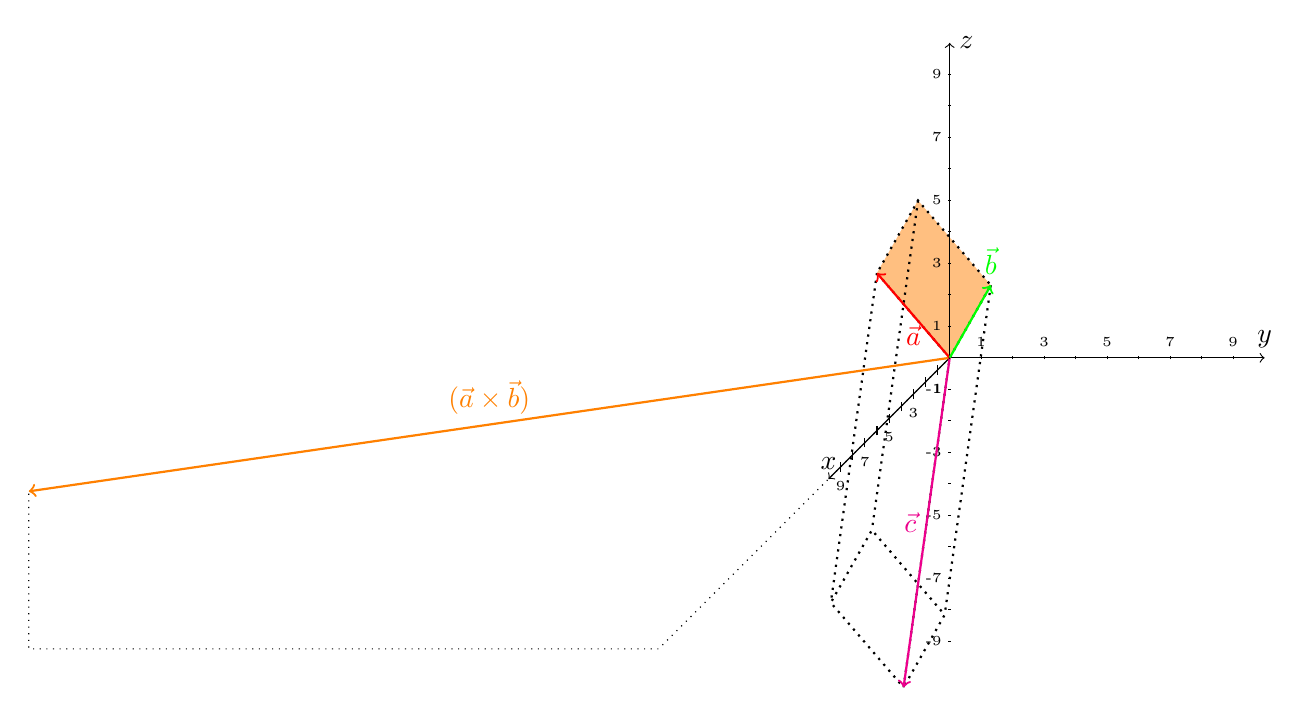
\begin{tikzpicture}[scale=0.4]

				\fill[orange!50]		(0,0,0) -- (0,5,6) -- (4, 10, 13) -- (4,5,7) -- cycle;

				\draw[->] (xyz cs:x=0) -- (xyz cs:x=10) node[above] {$y$};
				\draw[->] (xyz cs:y=0) -- (xyz cs:y=10) node[right] {$z$};
				\draw[->] (xyz cs:z=0) -- (xyz cs:z=10) node[above] {$x$};

				\foreach \coo in {-9, ...,9}
				{
					\draw (-1.5pt,\coo) -- (1.5pt,\coo);
				}
				\foreach \coo in {-9, -7, ..., 9}
				{
					\node at (1.5pt,\coo) [anchor = east]	{\tiny\coo};
				} 
				\foreach \coo in {1, ...,9}
				{
					\draw (\coo,-1.5pt) -- (\coo,1.5pt);
					\draw (xyz cs:y=-0.15pt,z=\coo) -- (xyz cs:y=0.15pt,z=\coo);
				}
				\foreach \coo in {1, 3, ..., 9}
				{
					\node at (\coo,1.5pt) [anchor = south]	{\tiny\coo};
					\node at (xyz cs:y=-0.15pt,z=\coo)
							      [anchor = north]	{\tiny\coo};
				} 

				\draw[dotted, thick] (0,0,0) -- (0,5,6) -- (4,10,13) -- (4,5,7) -- (0,0,0)
					-- (2,-7,9) -- (2,-2,15) -- (6,3,22) -- (6,-2,16) -- (2,-7,9);
				\draw[dotted, thick] (0,5,6) -- (2,-2,15);
				\draw[dotted, thick] (4,10,13) -- (6,3,22);
				\draw[dotted, thick] (4,5,7) -- (6,-2,16);
				\draw[->, orange, thick]	(0,0,0) -- node [anchor = south] {$(\vec a \times \vec b)$} (-20,5,24);
				\draw[->, red, thick]		(0,0,0) -- node [anchor = north] {$\vec a$} (0,5,6);
				\draw[->, green, thick]		(0,0,0) -- (4,5,7) node [anchor = south] {$\vec b$};
				\draw[->, magenta, thick]	(0,0,0) -- node [anchor = east] {$\vec c$}(2, -7, 9);
				\draw[dotted] (0,0,0) -- (0,0,24) -- (-20,0,24) -- (-20,5,24);
				%\draw[dotted] (0,0,0) -- (0,0,7) -- (4,0,7) -- (4,5,7);
		\end{tikzpicture}\\
		An dem Bild erkennt man, dass ${\color{orange}\left|\vec a \times \vec b\right|}$ gleich der Grundfläche vom Parallelepiped ist. Da die Richtung von $\vec a \times \vec b$ orthogonal zu der Grundfläche steht, ist die Abbildung von $\vec c$ auf $\vec a \times \vec b $ die Höhe des Parallelepipeds und $ c \cdot \left( \vec a \times \vec b \right) $ ist das Volumen.
\end{enumerate}

\section{Vektoraddition}
\begin{enumerate}[label=\alph*)]
	\item Damit der Schwimmer die kürzeste Strecke nimmt, muss seine Bahnkurve den kürzesten Weg von einem Ufer zu anderen Beschreiben, d.h. die Vektoren $\vec v_F $ und $ \vec v $ müssen summiert längs dem kürzesten Weg von einem Ufer zum anderen sein, also orthogonal zur Bewegungsrichtung des Wassers. Also gilt $\left(\vec v + \vec v_F\right) \cdot \vec v_F = 0 $:
		\begin{align*}
			0 &= \left( \vec v + \vec v_F \right) \cdot \vec v_F\\
			0 &= \vec v \cdot \vec v_F + \left(\vec v_F \right)^2\\
			0 &= ||\vec v|| \, ||\vec v_F|| \cos(\alpha) + \left(\qty{0.5}{\metre\per\second}\right)^2\\
			0 &= \qty{0.5}{\square\metre\per\square\second} \cos(\alpha) + \qty{0.25}{\square\metre\per\square\second}\\
			\qty{-0.25}{\square\metre\per\square\second} &= \qty{0.5}{\square\metre\per\square\second} \cos(\alpha)\\
			-0.5 &= \cos(\alpha)\\
			\arccos(-0.5) &= \alpha\\
			\alpha &= \frac{2\pi}{3}
		\end{align*}
		Wenn $\alpha = \frac{2\pi}{3}$, dann ist $ |\vec v_{\text{res}}| = \sqrt{\left(\qty{1}{\metre\per\second}\right)^2 - \left(\qty{0.5}{\metre\per\second} \right)^2} = \sqrt{0.75}\,\unit{\metre\per\second} $, also braucht der Schwimmer $\frac{\qty{156}{\metre}}{\sqrt{0.75}\,\unit{\metre\per\second}} \approx \qty{180}{\second}$. Er brauch also etwa 3 Minuten.
	\item $\sqrt{\left(\qty{1}{\metre\per\second}\right)^2 + \left(\qty{0.5}{\metre\per\second}\right)^2} = \sqrt{1.25}\,\unit{\metre\per\second} $

\end{enumerate}
\end{document}
